\documentclass[addpoints]{exam}

\usepackage{epic,array,ecltree,url}
\usepackage[nointegrals]{wasysym}

\usepackage{array,epsfig}
\usepackage{amsmath}
\usepackage{amsfonts}
\usepackage{amssymb}
\usepackage{amsxtra}
\usepackage{amsthm}
\usepackage{mlextra} % must be below ams packages
\usepackage{mathrsfs}
\usepackage{color}
\usepackage{array}
\usepackage{graphicx}
\graphicspath{ {../art/} }
\usepackage{bm}
\usepackage{tikz}
\usepackage{multicol}

%Pagination stuff.
\setlength{\topmargin}{-.3 in}
\setlength{\oddsidemargin}{0in}
\setlength{\evensidemargin}{0in}
\setlength{\textheight}{9.in}
\setlength{\textwidth}{6.5in}

\newcommand{\tf}[1][{}]{%
\fillin[#1][0.25in]%
}


\pointsinmargin
\begin{document}


\noindent
\begin{tabular*}{\textwidth}{l @{\extracolsep{\fill}} r @{\extracolsep{6pt}} l}
	{\large CS3920: Foundations of Computer Science} &  \makebox[3in]{\large Name:\enspace\hrulefill}\\
	%{Points: /\numpoints\. } \\
	%{\large June 8, 2018} & \\
	{\large Quiz 2} & \\
	{\large Points: \hspace{1cm}/\numpoints} & 
\end{tabular*}\\

\fbox{\fbox{\parbox{6in}{\textbf{Instructions}: Please answer the questions 
  below to the best of your ability. Be sure to show your work where appropriate. 
   This exam is closed book, closed notes, closed computer. There are \numpoints\ 
   points in total with points denoted in parentheses.
%    and \numbonuspoints\ possible extra credit points. 
    }}}\\
\begin{questions}

\question[4]
Prove $\emptyset^* = \{\epsilon\}$.

\vspace{40mm}

%\question
Recall the Post System for rooted trees:

\begin{tabular}{ll}
\bid{B} & $\id{nil} \in \id{RTL}$ \\
\bid{R1} & \underline{$t \in \id{RT} \hspace{4mm} l \in \id{RTL}$} \\ 
%\cline{2-4}  \\
& $\id{cons}(t, l) \in \id{RTL}$ \\
\bid{R2} & $l \in \id{RTL}$ \\ 
%\cline{2-4}  \\
& $\overline{\id{node}(l) \in \id{RT}}$ \\
\end{tabular}


%\begin{parts}



\question[5] Draw the structure that corresponds to the following {rooted tree}:\\

$\id{node}(\id{cons}(\id{node}(nil),\id{cons}(\id{node}(\id{cons}(\id{node}(nil), nil)), nil)))$



%\end{parts}
\vspace{60mm}


%\question[3] Let $S = \{a^{2k} | k \in \N_0 \}$ and let $T = \{a^{4k} | k \in
%\N_0\}$. Prove $T \subseteq S$.
%\vspace{25mm}

\clearpage




\question Given the Post system below, 
\begin{tabbing}
{\bf R2}XX \=  \kill
{\bf B1} \>
        \(\begin{array}[t]{l}
        p \in A
        \end{array}\) \\[2ex]
{\bf B2} \>
        \(\begin{array}[t]{l}
        q \in A
        \end{array}\) \\[2ex]
{\bf R1} \>
        \(\begin{array}[t]{l}
        x \in A \\
        \hline
        (\ngg x) \in A
        \end{array}\) \\[2ex]
{\bf R2} \>
        \(\begin{array}[t]{l}
        x \in A \;\;\;y \in A \\
        \hline
        (x \land y) \in A
        \end{array}\) 
\end{tabbing}
\begin{parts}
\part[2] What is the derivation height of $ (\ngg (\ngg p))$?
\vspace{10mm}
\part[5] Prove $((\ngg (p \land q)) \land q) \in A$ (i.e. show the derivation).
\end{parts}
\clearpage
%\question Let $L$ be the language of strings accepted by the automaton
%described in the state diagram below.
%
%\begin{center}
%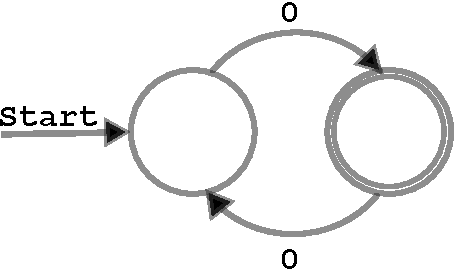
\includegraphics[width=2.5in, height=.75in,keepaspectratio=true]{oddzeroautomaton.pdf}
%\end{center}     
%\begin{parts}
%\part[1] What is the alphabet of $L$?
%\vspace{10mm}
%
%\part[2] Give a set comprehension for $L$. 
%\vspace{10mm}
%\end{parts}

\question Let $\sim$ be a relation on $\Sigma = \{0,1\}$, where $x\sim y$ for $x,y \in
\Sigma$ if and only if it is not the case that $x = 1$ and $y = 0$. 

\begin{parts}
\part[3] We claim that $\sim$ is a partial order on $\Sigma$. What properties
of $\sim$ must be established to prove this claim is true? (Do not prove them).

\vspace{10mm}

\part[5] Draw a digraph of  $\sim$  and explain why it shows transitivity.

\vspace{60mm}

\end{parts}

\question[4] Let $K$ be a set containing \emph{all} strings of odd length over the 
alphabet $\Sigma = \{a\}$.  Give a Post system for $K$.
\vspace{50mm}


\question The following Post system describes \textbf{full binary trees}:

\begin{tabbing}
	{\bf R2}XX \=  \kill
	{\bf B} \>
	\(\begin{array}[t]{l}
	\id{nil}\in\id{RTL}
	\end{array}\) \\[2ex]
	{\bf R1} \>
	\(\begin{array}[t]{l}
	t\in\id{RT}\;\;\;u\in\id{RT} \\
	\hline
	\id{cons}(t,u)\in\id{RTL}
	\end{array}\) \\[2ex]
	{\bf R2} \>
	\(\begin{array}[t]{l}
	l\in\id{RTL} \\
	\hline
	\id{node}(l)\in\id{RT}
	\end{array}\)
\end{tabbing}

\begin{parts}
	\part[1] \tf[T] (T/F) Only the empty list has a derivation height of zero.
	\part[1] \tf[T] (T/F) If $l \in \id{RTL}$ has a derivation height of $2$, the total
	number of leaf nodes in $l$ is $2$.
	%\part[1] \tf[F] (T/F) If $l \in \id{RTL}$ has a derivation height of $4$, it contains
	%two trees, each of which has a derivation height of $3$.
	\part[1] \tf[F] (T/F) If $t \in \id{RT}$ has a derivation height of $4$, it contains
	two subtrees, each of which has a derivation height of $3$.
	
	%\part[3] Draw the structure produced in the following derivation:\\
	
	%\begin{tabular}{llllll}
	%           &                                   & $\bid{B}$  & $\id{nil} \in \id{RTL}$            &\multicolumn{1}{r}{$\bid{B}$} & $\id{nil} \in \id{RTL}$                       \\ 
	%\cline{4-4}\cline{6-6}
	%           &                                   & $\bid{R2}$ & $\id{node}(\id{nil}) \in \id{RT}$  &\multicolumn{1}{r}{$\bid{R2}$} & $\id{node}(\id{nil}) \in \id{RT}$           \\
	%\cline{4-4}\cline{6-6}
	%$\bid{B}$  & $\id{nil} \in \id{RTL}$           & $\bid{R1}$ & \multicolumn{3}{l}{$\id{cons}(\id{node}(\id{nil}), \id{node}(\id{nil})) \in \id{RTL}$}  \\
	%\cline{2-2}\cline{4-6}
	%$\bid{R2}$ & $\id{node}(\id{nil}) \in \id{RT}$ & $\bid{R2}$ & \multicolumn{3}{l}{$\id{node}(\id{cons}(\id{node}(\id{nil}), \id{node}(\id{nil}))) \in \id{RT}$}  \\
	%\cline{2-6}
	%$\bid{R1}$ & \multicolumn{4}{l}{$\id{cons}(\id{node}(\id{nil}), \id{node}(\id{cons}(\id{node}(\id{nil}), \id{node}(\id{nil})))) \in \id{RTL}$}  &
	%\end{tabular}
	%\vspace{40mm}
	%\bonuspart[2] \tf[T] (T/F) If $t \in RT$ has a derivation height of $8$, it has the form $node(l)$, where $l$ has a 
	%              derivation height of $6$. To receive credit, you must answer
	%              correctly and give a brief justification of your answer:
	%\end{parts}
	
	
	%\vspace{40mm}
	%\bonuspart[2] \tf[T] (T/F) If $t \in RT$ has a derivation height of $8$, it has the form $node(l)$, where $l$ has a 
	%derivation height of $6$. To receive credit, you must answer
	%correctly and give a brief justification of your answer:
\end{parts}

%\vspace{20mm}


%\question
%Let $\Sigma = \{0,1,2\}$.  Let $T = \{t \in \Sigma^* | |t| \geq 3\}$.
%Now define $Z$ to be a relation on $T$ such that $xZy$ for $x,y \in T$ if and only if 
%there exist strings $r,s,m \in \Sigma^*$ such that $|m| = 3$ and $x = rm$ and $y = sm$. 
%
%\begin{parts}
%\part [3] We claim that $Z$ is an equivalence class on $T$. What properties of
%$Z$ must be established to prove this claim is true?
%\vspace{10mm}
%\part [2] Assume the claim is proven. How many equivalence classes are there with respect to $Z$?
%\vspace{10mm}
%\end{parts}

\clearpage
\question Consider the following Post System and answer (a), (b) and (c) below:
\begin{tabbing}
{\bf R2}XX \=  \kill
{\bf B} \>
        \(\begin{array}[t]{l}
        a \in D
        \end{array}\) \\[2ex]
{\bf R} \>
        \(\begin{array}[t]{l}
        x \in D \\
        \hline
        xx \in D
        \end{array}\) 
\end{tabbing}

Suppose you are asked to prove the following theorem:\\
If $x \in D$ then $|x| = 2^n$, where $n$ is the derivation height
of $x$.\\
\begin{parts}

\part[2] Which of the following induction rules should you choose?

\begin{choices}

\choice 
	\(\begin{array}[t]{l}
	S(i) \;\wedge\; S(i+1)\;\wedge\cdots\wedge\;S(j)\;\wedge\; \\
\forall n \geq j.\;S(i)\;\wedge\;S(i+1)\;\wedge\cdots\wedge\;S(n) \Rightarrow S(n+1) \\
	\hline
	\forall n \geq i. \; S(n)
	\end{array}\) % \\[2ex]


\choice 
	\(\begin{array}[t]{l}
	S(i) \;\lor\; \forall k \leq i.\;S(i)\;\wedge\;S(i+k)\;\lor\cdots\lor\;S(n) \Rightarrow S(n+1) \\
	\hline
	\forall n \leq i. \; S(n)
	\end{array}\)

\choice 
	\(\begin{array}[t]{l}
	S(i) \;\wedge\; \forall n \geq i.\;S(n) \Rightarrow S(n+1) \\
	\hline
	\forall n \geq i. \; S(n)
	\end{array}\) % \\[2ex]
\choice 
	\(\begin{array}[t]{l}
	S(i) \;\wedge\; \forall n \geq i.\;S(i)\;\wedge\;S(i+1)\;\wedge\cdots\wedge\;S(n) \Rightarrow S(n+1) \\
	\hline
	\forall n \geq i. \; S(n)
	\end{array}\)

\end{choices}
\part [2] Briefly justify your answer to part (a):
\vspace{20mm}

%\clearpage

\part[3] Prove the base case (or base cases).
\vspace{30mm}

%
%\part[2] Is this a soundness or completeness result of the theorem?
%\vspace{5mm}

\end{parts}
%\clearpage

\clearpage

%\clearpage
%\question[3] Let $L$ be the language of strings accepted by the automaton
%described in the diagram below, and let $R$ and $Q$ be sets defined by
%the Post system given on the right.
%
%\begin{multicols}{2}
%\begin{center}
%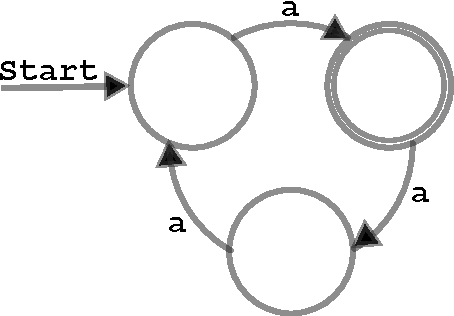
\includegraphics[width=2.5in, height=1in,keepaspectratio=true]{1mod3automaton.pdf}
%
%\end{center}
%
%\begin{tabbing}
%{\bf R2}XX \=  \kill
%{\bf B} \>
%        \(\begin{array}[t]{l}
%        a \in R
%        \end{array}\) \\[2ex]
%{\bf R1} \>
%        \(\begin{array}[t]{l}
%        x\in R  \\
%        \hline
%        xaa \in Q
%        \end{array}\) \\[2ex]
%{\bf R2} \>
%        \(\begin{array}[t]{l}
%        x\in R\;\;\;y\in Q \\
%        \hline
%        xy \in R
%        \end{array}\) 
%\end{tabbing}
%\end{multicols}
%
%%Consider the claim that $L = \{a^{3k +1} | k \in
%%\N_0 \}$.  Suppose you are asked to prove that the automata accepts \emph{all}
%%strings in $L$ by induction on $k$.\\
%%\begin{parts}
%%\part[2] Write out the two shortest strings contained in the set $R$.
%%\vspace{10mm}
%
%%\part[3]
% Give a set comprehension for $L$. 
%%\vspace{10mm}
%
%%\part[4] We claim that if a string in $R$ has derivation height $n$, it is accepted
%%by the automaton. Prove this claim holds for $n=0$ and $n=1$.
%%\vspace{25mm}
%%
%%\part[4] We claim that if a string in $Q$ has a derivation height $n$, this string 
%%will put the automaton in the start state.  Prove this claim holds 
%%for $n=0$ and $n=1$.
%%\vspace{25mm}
%%
%%\part[3] Suppose you are asked to prove, by induction on derivation height, that
%%all strings in $R$ are accepted by the automaton (i.e, $R \subseteq L$).  
%%Which of the following induction rules should you choose?
%%\begin{choices}
%%
%%\choice 
%%	\(\begin{array}[t]{l}
%%	S_1(i)\;\wedge\;S_2(i)\;\wedge\;\forall n \geq i.\;S_1(n)\;\wedge\;S_2(n)\Rightarrow S_1(n+1)\;\wedge\;S_2(n+1)\\
%%	\hline
%%	\forall n \geq i. \; S_1(n)\;\wedge\;S_2(n)
%%	\end{array}\) % \\[2ex]
%%
%%\choice 
%%	\(\begin{array}[t]{l}
%%	S_1(i) \;\wedge\;S_2(i) \;\wedge\; \forall n \geq i.\;S_1(i)\;\wedge\;S_2(i)\;\wedge\cdots\wedge\;S_1(n)\;\wedge\;S_2(n)\Rightarrow S_1(n+1)\;\wedge\;S_2(n+1)\\
%%	\hline
%%	\forall n \geq i. \; S_1(n)\;\wedge\;S_2(n)
%%	\end{array}\)
%%
%%\choice 
%%	\(\begin{array}[t]{l}
%%	S(i) \;\wedge\; \forall n \geq i.\;S(n) \Rightarrow S(n+1) \\
%%	\hline
%%	\forall n \geq i. \; S(n)
%%	\end{array}\) % \\[2ex]
%%
%%\choice 
%%	\(\begin{array}[t]{l}
%%	S_1(i) \;\wedge\; S_2(i)\;\wedge\;S_1(i+1) \;\wedge\; S_2(i+1)\;\wedge\;\cdots\wedge\;S_1(j)\;\wedge\;S_2(j) \\
%%\forall n \geq
%%j.\;S_1(i)\;\wedge\;S_2(i)\;\wedge\cdots\wedge\;S_1(n)\wedge\;S_2(n)\Rightarrow S_1(n+1)\wedge\;S_2(n+1)\\
%%	\hline
%%	\forall n \geq i. \; S_1(n)\;\wedge\;S_2(n)
%%	\end{array}\) % \\[2ex]
%%
%%
%%\end{choices}
%%\part[2] Briefly justify your answer to part (a):
%%\vspace{25mm}
%%
%%\vspace{35mm}
%
%%\end{parts}
%\clearpage

\question[5]

Recall the Post System for full binary trees:

\begin{tabular}{ll}
	\bid{B} & $\id{nil} \in \id{RTL}$ \\
	\bid{R1} & \underline{$t \in \id{RT} \hspace{4mm} u \in \id{RT}$} \\ 
	%\cline{2-4}  \\
	& $\id{cons}(t, u) \in \id{RTL}$ \\
	\bid{R2} & $l \in \id{RTL}$ \\ 
	%\cline{2-4}  \\
	& $\overline{\id{node}(l) \in \id{RT}}$ \\
\end{tabular}

Consider the following claim:
If $t \in \id{RT}$ then $N_{\id{edges}(t)}=N_{\id{nodes}(t)} -1$

Where 

\hspace{1cm} $N_{\id{edges}(t)}$ denotes the number of edges in the tree $t$ and 

\hspace{1cm} $N_{\id{nodes}(t)}$ denotes the number of nodes in the tree $t$.\\



\begin{proof}


Induction Hypothesis:

$S_1(n): $  $N_{\id{edges}(t)}=N_{\id{nodes}(t)} -1$   for tree $t$ of derivation height $n$.

$ S_2(n): $  $N_{\id{edges}(l)}=N_{\id{nodes}(l)} -|l|$ for list $l$ of derivation height $n$. \\

Base Step:

Prove $S_1(0), S_1(1), S_1(2)$:
\textit{\color{blue}(proof omitted)}

Prove $S_2(0), S_2(1), S_2(2)$:
\textit{\color{blue}(proof omitted)} \\

Induction Step:

Assume $S_1(0) \land \ldots \land S_1(n)$. Show $S_1(n+1)$.
\textit{\color{blue}(proof omitted)} \\

 


Assume $S_2(0) \land \ldots \land S_2(n)$. Show $S_1(n+1)$.

\textbf{\color{blue} Justify each step of the proof of the above statement in the provided space. }\\


Suppose $l' \in \id{RTL}$ has derivation height $n+1$ where $n\geq 0$. Then \\
%\begin{parts}



\begin{tabular}{llrl}
		\vspace{5mm}
		
	$l' = \id{cons}(t, u)$ & where $t, u$ have derivation height $\leq n$. &\hspace{15mm}  {\color{blue}(1 point)}& {\color{blue}\underline{\hspace{4cm}} } \\
	\vspace{5mm}
	
	 $N_{\id{edges}(l)}$ = & $N_{\id{edges}(t)} + N_{\id{edges}(u)}$   & {\color{blue}(1 point)}& {\color{blue}\underline{\hspace{4cm}} } \\
	 	\vspace{5mm}
	 	
	%\cline{2-4}  \\
	& $N_{\id{nodes}(t)} -1 + N_{\id{nodes}(u)} -1$  & {\color{blue}(1 point)}& {\color{blue}\underline{\hspace{4cm}} } \\
		\vspace{5mm}

	& $N_{\id{nodes}(l')} -2$  & {\color{blue}(1 point)}& {\color{blue}\underline{\hspace{4cm}} } \\
		\vspace{5mm}
		
	& $N_{\id{nodes}(l')} -|l'|$  & {\color{blue}(1 point)}& {\color{blue}\underline{\hspace{4cm}} }
\end{tabular}

\end{proof}

%Prove injective / surjective.
%Prove a partial order.
%Prove an equivalence relation.
%Give a Post System.
%Prove an element is in a Post system.
%
%Read a derivation and describe the object.
%Prove a property of full binary trees or extended binary trees.
%Read a proof and choose the correct induction rule.



%\newpage

\end{questions}
\end{document}


